\documentclass[12pt]{article}
\usepackage[top=1in, bottom=1in, left=.75in, right=.75in]{geometry}
\usepackage{amsmath, enumerate}
\usepackage{fancyhdr}
\usepackage{graphicx, xcolor, setspace}
\usepackage{txfonts}
\usepackage{multicol,coordsys,pgfplots}
\usepackage[scaled=0.86]{helvet}
\renewcommand{\emph}[1]{\textsf{\textbf{#1}}}
\usepackage{anyfontsize}
% \usepackage{times}
% \usepackage[lf]{MinionPro}
\usepackage{tikz,pgfplots}
\def\ra{\rightarrow}
\newcommand{\blank}[1]{\rule{#1}{0.75pt}}
\usetikzlibrary{calc,trees,positioning,arrows,fit,shapes,calc}
\pgfplotsset{width=9cm,compat=1.9}
\tikzset{
  jumpdot/.style={mark=*,solid},
  excl/.append style={jumpdot,fill=white},
  incl/.append style={jumpdot,fill=black},
}

\pgfplotsset{my style/.append style={axis x line=middle, axis y line=
middle, xlabel={$x$}, ylabel={$y$}}}

%axis equal

%yticklabels={,,} , xticklabels={,,}

% \setmainfont{Times}
% \def\sansfont{Lucida Grande Bold}
\parindent 0pt
\parskip 4pt
\pagestyle{fancy}
\fancyfoot[C]{\emph{\thepage}}
\fancyfoot[R]{v1} %%%%%% <-- Version Info
\fancyhead[L]{\ifnum \value{page} > 1\relax\emph{Math F251X: Midterm 1}\fi}
\fancyhead[R]{\ifnum \value{page} > 1\relax\emph{Spring 2025}\fi}
\headheight 15pt
\renewcommand{\headrulewidth}{0pt}
\renewcommand{\footrulewidth}{0pt}
\let\ds\displaystyle
\def\continued{{\emph {Continued....}}}
\def\continuing{{\emph {Problem \arabic{probcount} continued....}}\par\vskip 4pt}


\newcounter{probcount}
\newcounter{subprobcount}
\newcommand{\thesubproblem}{\emph{\alph{subprobcount}.}}
\def\problem#1{\setcounter{subprobcount}{0}%
\addtocounter{probcount}{1}{\emph{\arabic{probcount}.\hskip 1em(#1)}}\par}
\def\subproblem#1{\par\hangindent=1em\hangafter=0{%
\addtocounter{subprobcount}{1}\thesubproblem\emph{#1}\hskip 1em}}
\def\probskip{\vskip 10pt}
\def\medprobskip{\vskip 2in}
\def\subprobskip{\vskip 45pt}
\def\bigprobskip{\vskip 4in}


\newenvironment{subproblems}{%
\begin{enumerate}%
\setcounter{enumi}{\value{subprobcount}}%
\renewcommand{\theenumi}{\emph{\alph{enumi}}}}%
{\setcounter{subprobcount}{\value{enumi}}\end{enumerate}}


\newcommand{\be}{\begin{enumerate}}
\newcommand{\ee}{\end{enumerate}}


\begin{document}
{\emph{\fontsize{26}{28}\selectfont Spring 2025 \hfill
%{\fontsize{32}{36}\selectfont Calculus 1: Midterm 1}
\hfill Math F251X}}

\begin{center}
{\emph{%\fontsize{26}{28}\selectfont Spring 2024 
%%\hfill
{\fontsize{32}{36}\selectfont Calculus 1: Midterm 1}
%%\hfill Math F251X}
}}
\end{center}

%\vskip 2cm
\strut\vtop{\halign{\emph#\hskip 0.5em\hfil&#\hbox to 2in{\hrulefill}\cr
\emph{\fontsize{18}{22}\selectfont Name:}&\cr
%\noalign{\vskip 10pt}
%\emph{\fontsize{18}{22}\selectfont Student Id:}&\cr
%\noalign{\vskip 10pt}
%\emph{\fontsize{18}{22}\selectfont Calculator Model:}&\cr
}}
\hfill
\vtop{\halign{\emph{\fontsize{18}{22}\selectfont #}\hfil& \emph{\fontsize{18}{22}\selectfont\hskip 0.5ex $\square$ #}\hfil\cr
Section: & 9:15am (James Gossell)\cr
\noalign{\vskip 4pt}
         & 11:45am (Kevin Meek)\cr
\noalign{\vskip 4pt}
         & async (Deven Barnett)\cr}}

\vfill
{\fontsize{18}{22}\selectfont\emph{Rules:}}

\begin{itemize}
\item Partial credit will be awarded, but you must show your work.

\item You may have a single handwritten $3'' \times 5''$ notecard, both sides.

\item Calculators are {\bf not} allowed. 

\item Place a box around your  \fbox{FINAL ANSWER} to each question where appropriate.

\item Turn off anything that might go beep during the exam.

\end{itemize}

%If you need extra space, you can use the back sides of the pages.
%Please make it obvious  when you have done so.



Good luck!
\vfill
\def\emptybox{\hbox to 2em{\vrule height 16pt depth 8pt width 0pt\hfil}}
\def\tline{\noalign{\hrule}}
\centerline{\vbox{\offinterlineskip
{
\bf\sf\fontsize{18pt}{22pt}\selectfont
\hrule
\halign{
\vrule#&\strut\quad\hfil#\hfil\quad&\vrule#&\quad\hfil#\hfil\quad
&\vrule#&\quad\hfil#\hfil\quad&\vrule#\cr
height 3pt&\omit&&\omit&&\omit&\cr
&Problem&&Possible&&Score&\cr\tline
height 3pt&\omit&&\omit&&\omit&\cr
&1&&12&&\emptybox&\cr\tline
&2&&12&&\emptybox&\cr\tline
&3&&6&&\emptybox&\cr\tline
&4&&6&&\emptybox&\cr\tline
&5&&10&&\emptybox&\cr\tline
&6&&8&&\emptybox&\cr\tline
&7&&6&&\emptybox&\cr\tline
&8&&12&&\emptybox&\cr\tline
&9&&12&&\emptybox&\cr\tline
&10&&16&&\emptybox&\cr\tline \tline
&Extra Credit&&(5)&&\emptybox&\cr\tline
&Total&&100&&\emptybox&\cr
}\hrule}}}

\newpage
%Graph problem
\problem{12 points} Use the graph of $f(x)$ to answer the following questions.
%Begin picture
\begin{center}
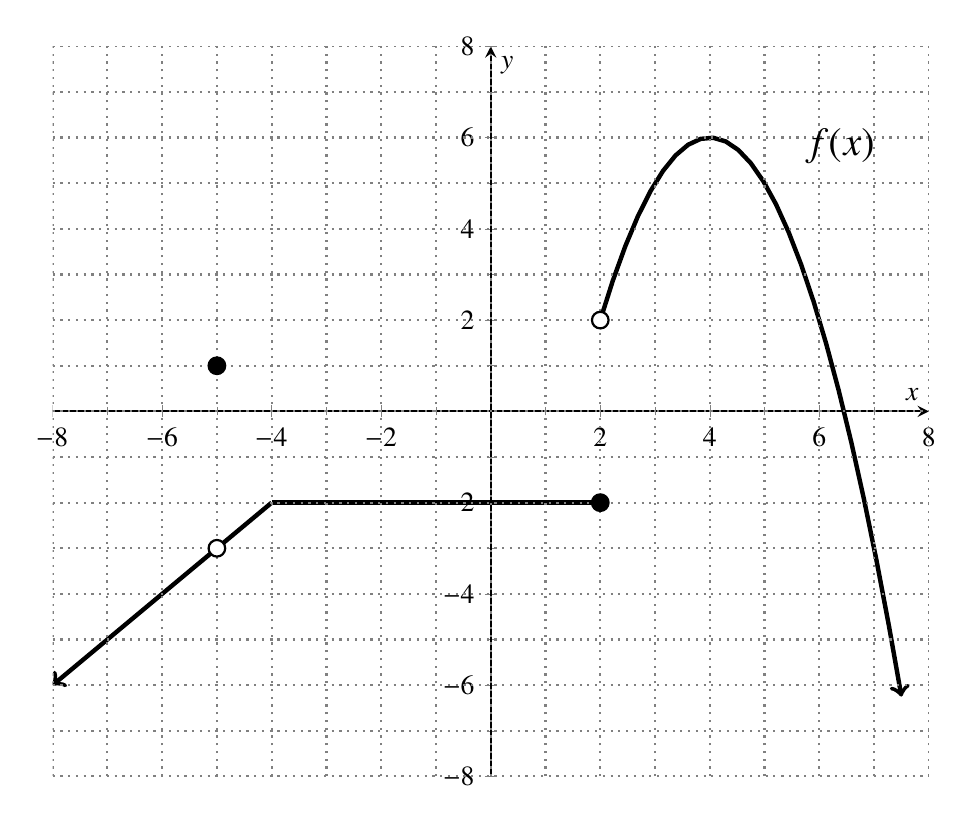
\begin{tikzpicture}
\begin{axis}[scale=1.5, thick, my style, xtick={-8,-6,...,8}, ytick={-8,-6,-4,-2,...,8},
xmin=-8, xmax=8, ymin=-8, ymax=8, minor y tick num=1,
        minor x tick num=1, mark size=3.0pt]
        \addplot[domain=-8:-4, smooth, ultra thick,<-] coordinates { (-8,-6) (-4,-2)};
        \addplot[domain=-4:-2, smooth, ultra thick] coordinates {  (-4,-2) (2,-2)};
        \addplot[ultra thick,domain=2:7.5,->]{3-(x-4)*(x-4)+3};
\foreach \i in {-8,-7,-6,...,8}{
	\addplot[dotted, gray, domain=-8:8]{\i};
	\addplot[dotted, gray] coordinates {(\i,-8) (\i,8)};
	}
\addplot[mark=*,only marks] coordinates {(2,-2)(-5,1)};
 \addplot[mark=*,fill=white,only marks] coordinates {(2,2)(-5,-3)};
\end{axis}
\node at (10,8){{\Large{$f(x)$}}};
\end{tikzpicture}
\end{center}
\subproblem{} Fill in the blanks below. If the value does not exist or is undefined, write DNE.\\

\begin{center} \begin{tabular}{lllll}
$\ds \lim_{x \to -5} f(x) =$ \blank{0.5in} && $f(-5)=$ \blank{0.5in} && $\ds \lim_{x \to -4} f(x) =$ \blank{0.5in}\\
&&&&\\
$\ds \lim_{x \to 2^{+}} f(x) =$ \blank{0.5in}&& $f(2)=$\blank{0.5in}&& $\ds \lim_{x \to 2} f(x) =$ \blank{0.5in}\\
&&&&\\
$\ds f'(-6)=$ \blank{0.5in}&& $f'(4)=$\blank{0.5in}&& $\ds \lim_{x \to -4^+} f'(x) =$ \blank{0.5in}\\
\end{tabular} \end{center}
\vfill
\subproblem{} State the $x$-values for which $f$ is \emph{not continuous}.\\
 

\vfill
	\subproblem{} State at least one $x$-value for which $f$ is \emph{not differentiable} (where $f'(x)$ does not exist).\\
	\vfill
\newpage

%Straight limit problems
\problem{12 points} Compute the following limits. Show your work and use limit notation where necessary. You will be graded both on your computation and your correct use of notation.

\begin{subproblems}

	\item $\ds \lim_{x \rightarrow 3} \frac{x^2-5x+6}{3-x}$
	
	\vfill

	\item $\ds \lim_{x \rightarrow 1} \frac{\text{ }1-\cfrac{1}{x^2}\text{ }}{x-1}$
	
	\vfill
	
	\item $\ds \lim_{x \rightarrow 4} \frac{\sqrt{x}+2}{x+4}$
	
	\vfill
\end{subproblems}

\newpage

% Continuity
\problem{6 points} Determine whether or not the given function is continuous
at $x=3$. {\bf Justify your answer using limits}.

   \begin{equation*}
    f(x) =
    \begin{cases}
      x^2-4 & \text{ if } x > 3 \\
      2x+1 & \text{ if } x \leq 3
    \end{cases}
  \end{equation*}

\vfill
\vfill

\problem{6 points} Find the value(s) of $k$ that make the function continuous at $x=-2$.
  
   \begin{equation*}
    g(x) =
    \begin{cases}
      \frac{x^2+3x+2}{x+2} & \text{ if } x \neq -2 \\
      k & \text{ if } x = -2
    \end{cases}
  \end{equation*}

\vfill
\vfill

\newpage

%\problem{1} Find the value(s) of $k$ that make the function continuous at $x=3$.

%   \begin{equation*}
%    f(x) =
%    \begin{cases}
%      x^2-k & \text{ if } x > 3 \\
%      4x+1 & \text{ if } x \leq 3
%    \end{cases}
%  \end{equation*}

\problem{10 points} Use the limit definition (given below) of the derivative
to find the derivative of $$\displaystyle f(x)=3x^2-4x.$$ Show
all your work clearly, step by step, using correct notation. \emph{No
credit will be awarded for a solution that does not use the definition
below.}\\
$$f'(x) = \lim_{h \to 0} \frac{f(x+h) - f(x)}{h}$$

% \problem{1} Use the limit definition (given below) of the derivative
% to find the derivative of $$\displaystyle f(x)=\sqrt{x+2}.$$ Show
% all your work clearly, step by step, using correct notation. \emph{No
% credit will be awarded for a solution that does not use the definition
% below.}\\
% $$f'(x) = \lim_{h \to 0} \frac{f(x+h) - f(x)}{h}$$

\vfill
\vfill
\vfill
\vfill
\vfill

\newpage

\problem{8 points} The function $y=H(x)$ is graphed below. Sketch the graph of $H'(x)$ on the blank set of axes provided.

\begin{multicols}{2}
\begin{center}
		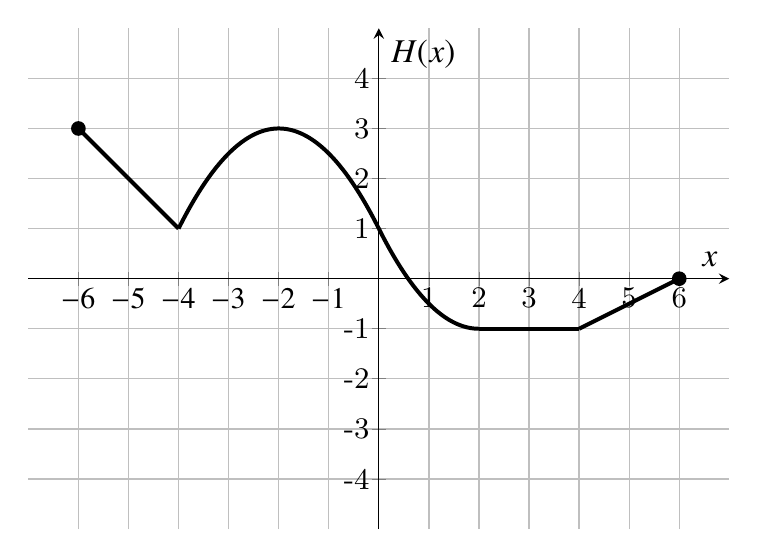
\begin{tikzpicture}[scale=1.2]
		\begin{axis}[
		axis lines=middle,
		unit vector ratio=1 1 1,
		grid=major,
		xmin=-7,
		xmax=7,
		ymin=-5,
		ymax=5,
		xlabel=$x$,
		ylabel=$H(x)$,
		xtick={-6,-5,...,5,6},
		xticklabels={ $-6$,$-5$,$-4$,$-3$,$-2$,$-1$,0,1,2,3,4,5, 6},
		ytick={-4,-3,...,3,4},
		yticklabels={-4,-3,-2,-1,0,1,2 ,3,4},
		yticklabel style = {xshift=0.1cm},
		xticklabel style = {yshift=0.1cm},
		tick label style={font=\small},
		legend style={
			at={(rel axis cs:0,1)},
			anchor=north west,draw=none,inner sep=0pt,fill=gray!10}
		]
		\addplot[-,domain=(-6:-4, black, very thick, samples=100] {-x-3};
		\addplot[-,domain=(-4:0, black, very thick, samples=100] {-(1/2)*(x+2)^2+3};
		\addplot[-,domain=(0:2, black, very thick, samples=100] {(1/2)*(x-2)^2-1};
		\addplot[-,domain=(2:4, black, very thick, samples=100] {-1};
		\addplot[-,domain=(4:6, black, very thick, samples=100] {x/2-3};
		\addplot[incl] coordinates {(-6,3)};
		\addplot[incl] coordinates {(6,0)};
		\end{axis}
		\end{tikzpicture}
\end{center}
%\vspace{2cm}

\begin{center}
		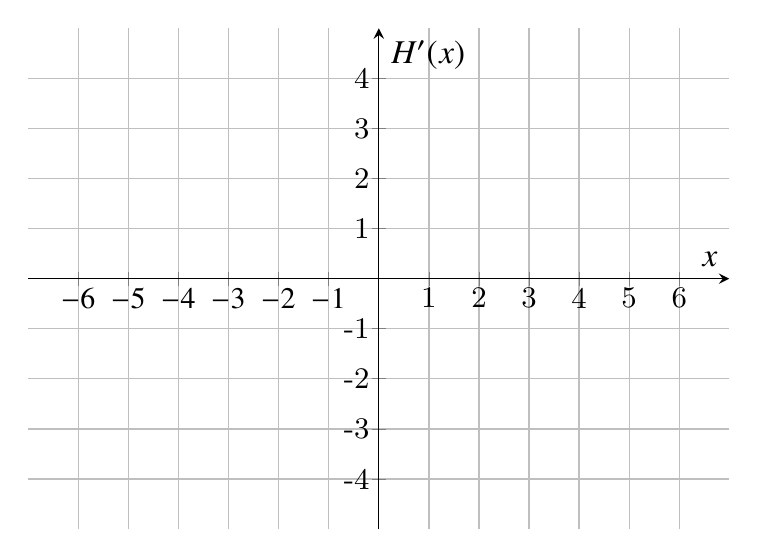
\begin{tikzpicture}[scale=1.2]
		\begin{axis}[
		axis lines=middle,
		unit vector ratio=1 1 1,
		grid=major,
		xmin=-7,
		xmax=7,
		ymin=-5,
		ymax=5,
		xlabel=$x$,
		ylabel=$H'(x)$,
		xtick={-6,-5,...,5,6},
		xticklabels={ $-6$,$-5$,$-4$,$-3$,$-2$,$-1$,0,1,2,3,4,5, 6},
		ytick={-4,-3,...,3,4},
		yticklabels={-4,-3,-2,-1,0,1,2 ,3,4},
		yticklabel style = {xshift=0.1cm},
		xticklabel style = {yshift=0.1cm},
		tick label style={font=\small},
		legend style={
			at={(rel axis cs:0,1)},
			anchor=north west,draw=none,inner sep=0pt,fill=gray!10}
		]
		\end{axis}
		\end{tikzpicture}
\end{center}
\end{multicols}

\vspace{1cm}

%Derivative Application
\problem{6 points} $S(t)$ is a function that describes the human population of Lewisburg, West Virginia $t$ years after 1970 when the population was first recorded.  
	\begin{subproblems}
	\item Interpret the meaning of \fbox{$S(10)=2570$} in the context of the problem. Write a sentence or two including appropriate units. 
	
	\vfill
	
	\item Interpret the meaning of \fbox{$S'(10)=-135$} in the context of the problem. Write a sentence or two including appropriate units. 
	
	\vfill
	
	\item Given $S(10)=2570$ and $S'(10) = -135$, \emph{estimate} $S(9)$ including units. Write a sentence explaning how you arrived at your estimation.
	
	\vfill
\end{subproblems}

  % \problem{1} What can you say about $f'(3)$ if $\ds f(x) = \frac{e^{\sin(4x^5-3x^2-1)}\ln(\sqrt{x+32})}{x-3}$? (maybe bonus?)

  % \problem{1} BONUS: Note that $\ds \tan\left(\frac{\pi}{3}\right) =
  % \sqrt{3}$ and $\ds \tan\left(\frac{5\pi}{3}\right) = -\sqrt{3}$. Does
  % the Intermediate Value Theorem guarantee that $f(x) = \tan(x)$ has a
  % zero on the interval $\ds
  % \left[\frac{\pi}{3},\frac{5\pi}{3}\right]$? Why or why not?


\newpage

%Straight derivative problems
\problem{12 points} For each of the following functions, compute the derivative. 
\emph{You do not need to simplify your answers.} Your answer must begin with $f'(x)$ or similar notation, as appropriate to the problem.
 
\begin{subproblems}
	\item $\displaystyle{f(x)=\frac{x^3+3x^2+2}{\sqrt{x}}}$
	\vfill
	\item $\displaystyle{g(y)=y^{-6}\cos(y) + 5^2 - 4\pi y}$
	\vfill
	\item $\displaystyle{g(\theta) = \frac{\cos(\theta)}{\sin(\theta)}}$
	\vfill
\end{subproblems}


\newpage


%%%%%  tangent lines
\problem{12 points} Consider the function 
$\ds g(x) = \frac{1}{x^2}+\frac{x^4}{4} .$

\begin{subproblems}

 \item Find $g'(x)$. 
  (Use differentiation rules, not the definition of the derivative.)
  
\vfill
  
  \item Determine the $x$-values for which the function has a horizontal tangent line.
  
  \vfill
  
   \item Is the function increasing or decreasing at $x=-2$?  Show your work. 
   
  \vfill
  
 \item Find the equation of the tangent line to $g(x)$ at $x=-2$.
 
 
  \vfill
\end{subproblems}


\newpage
%%%%%%%%%% velocity and stuff




\problem{16 points} The position of a lady bug on a branch is given by $P(t) = t^3 -\frac{11}{2}t^2+6t+8$ where time $t$ is in minutes between $0$ and $20$ and position $P(t)$ is in inches. 
	\begin{subproblems}
	\item Find the function describing the \emph{velocity} of the lady bug.
	
	\vfill
	
	\item At what times did the lady bug stop moving?
	
	\vfill
	
	\item $P(t)$ is measured from the trunk of the tree meaning $P(t)=0$ indicates that the lady bug is at the trunk, the base of the branch. At time $t=2$ minutes, is the lady bug moving away from the trunk or towards the trunk? Show your work.
	
	\vfill
	
	\item At time $t=2$ minutes, is the lady bug speeding up or slowing down? Explain.
	
	\vfill 
	\end{subproblems}

\newpage


%\fbox{Extra Credit} 
\problem{Extra Credit: 5 points} 

Find a point on the graph of $f(x) = x^2 + x -1$ such that the tangent line at that point has a $y$ intercept at $(0,-2)$. 
\vfill


\end{document}

%%%%ENDDOCUMENT


